
\textbf{Segurança Cibernética em Smart Metering :}

O palestra ministrada por um funcionário de Inmetro destacou as dificultades de
se avaliar os novos sensores, onde, além do hardware que faz a medida, existe,
por trás, um software que pode influenciar no valor que é medido.

Dentre as tecnolgias exploradas para a validação do software e posterior
auditoria, foram destacadas as seguintes: \textit{Charles Response}, Ofuscação
de Código, FingerPrinting (geração de marcas d'água no software) e
Rastreabilidade, que é a técnica de conferir a relação entre o código fonte
aprovado e o binário implementado, sendo, em geral, feita através de marcadores.

Ao final, o palestrante citou que está sendo estudado um hardware, baseado em
tecnologia ARM, referido como ``Chip Inmetro'', que servirá para implementar
todas as medidas de segurança instituidas pelo Inmetro. Facilitando tanto a
validação do Inmetro, quanto a implementação por parte do fabricante,
figura~\ref{fig::inmetro}.

\begin{figure}[h!]	
	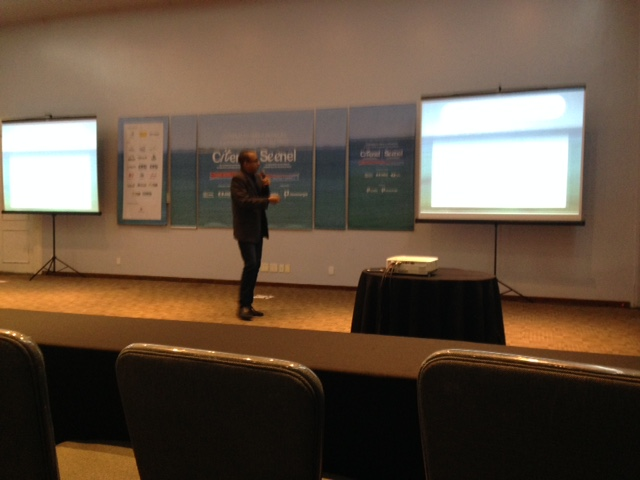
\includegraphics[width=\columnwidth]{figs/inmetro.JPG}
	\caption{Ilustração da palestra Segurança Cibernética em Smart Metering.}
	\label{fig::inmetro}
\end{figure}